% !TEX encoding = UTF-8 Unicode

%%%%%%%%%%%%%%%%%%%% author.tex %%%%%%%%%%%%%%%%%%%%%%%%%%%%%%%%%%%
%
% sample root file for your "contribution" to a proceedings volume
%
% Use this file as a template for your own input.
%
%%%%%%%%%%%%%%%% Springer %%%%%%%%%%%%%%%%%%%%%%%%%%%%%%%%%%


\documentclass[conference]{IEEEtran}
%
% RECOMMENDED %%%%%%%%%%%%%%%%%%%%%%%%%%%%%%%%%%%%%%%%%%%%%%%%%%%
%

% to typeset URLs, URIs, and DOIs
% https://www.overleaf.com/learn/latex/Hyperlinks
\usepackage{hyperref}
\hypersetup{
    colorlinks=true,
    linkcolor=blue,
    filecolor=magenta,      
    urlcolor=cyan,
    pdftitle={Overleaf Example},
    pdfpagemode=FullScreen,
    }

\def\UrlFont{\rmfamily}

\usepackage[T1]{fontenc}
\usepackage[utf8]{inputenc}
\usepackage[textsize=scriptsize]{todonotes}
\usepackage{gensymb}
\usepackage{array,multirow}
\usepackage{caption} 
\usepackage{subcaption}
\captionsetup[table]{skip=10pt}
\usepackage{makecell}

\usepackage{cite}
\usepackage{amsmath,amssymb,amsfonts}
\usepackage{bm}
\usepackage{algorithmic}
\usepackage{graphicx}
\usepackage{textcomp}
\usepackage{xcolor}
\def\BibTeX{{\rm B\kern-.05em{\sc i\kern-.025em b}\kern-.08em
    T\kern-.1667em\lower.7ex\hbox{E}\kern-.125emX}}

\usepackage{graphicx}
\graphicspath{ {./img/} }

\renewcommand{\labelenumii}{\theenumii}
\renewcommand{\theenumii}{\theenumi.\arabic{enumii}.}

\begin{document}
%
\title{Application of PID controller and CNN to control Duckiebot robot}
% \title{Application of PID and CNN controllers to control the Duckiebot robot}


\author{
\IEEEauthorblockN{1\textsuperscript{st} Marek Długosz}
\IEEEauthorblockA{\textit{AGH University of Science and Technology}\\
Cracow, Poland \\
mdlugosz@agh.edu.pl \\
0000-0001-6827-9149}\\[0.4cm]
\IEEEauthorblockN{3\textsuperscript{rd} Marcin Szelest}
\IEEEauthorblockA{\textit{IEEE Senior Member}}
\IEEEauthorblockA{\textit{AGH University of Science and Technology} \\
Cracow, Poland \\
mszelest@agh.edu.pl\\
0000-0002-0522-1270}
\and
\IEEEauthorblockN{2\textsuperscript{nd} Paweł Skruch}
\IEEEauthorblockA{\textit{IEEE Senior Member}}
\IEEEauthorblockA{\textit{AGH University of Science and Technology} \\
Cracow, Poland \\
pawel.skruch@agh.edu.pl\\
0000-0002-8290-8375}\\
\IEEEauthorblockN{4\textsuperscript{th} Artur Morys-Magiera}
\IEEEauthorblockA{\textit{AGH University of Science and Technology} \\
Cracow, Poland \\
amorys@student.agh.edu.pl\\
0000-0002-2137-8841}
}


\maketitle              % typeset the title of the contribution

\begin{abstract}

\end{abstract}


% We would like to encourage you to list your keywords within
% the abstract section using the \keywords{...} command.
\begin{IEEEkeywords}
autonomouse robot, PID controller, convolutional neural network, line follower
\end{IEEEkeywords}
%
\section{Introduction}
Recent years have seen a kind of renaissance in the use of artificial neural networks. Various types of network architectures have been created and are generally available, their training methods have been improved. All this has led to the fact that artificial neural networks are increasingly used, with success, in automatic control systems \cite{algor2030973, 786109}. The use of neural networks in automation systems is not their typical use because very often control can be implemented using well-known and described classical control algorithms (PID, LQR, MPC, etc.). This provides an opportunity to compare the performance of two different technologies, to find their advantages and disadvantages. In the process of educating students, the design and implementation by them of a control system using classical control algorithms and artificial neural networks is very interesting from both a scientific and didactic point of view.

An important element of student education that increases the attractiveness of the classes themselves, providing the opportunity to solve practical problems, is the use of real robots. One such project providing a complete robotics platform (hardware, software, simulator, teaching materials) is the Duckietown project.
The Duckietown project was created in 2016 at the University of Massachusetts Institute of Technology (MIT) as part of a class for students \cite{paull2017duckietown}. It is an open project that aims to promote education and research related to robot autonomy, especially in the context of autonomous cars. As part of the project, Duckiebot robots, mock-ups of the Duckietown cities the robots navigate through, and additional infrastructure, such as the Watchtower, to support the navigation process, have been created. 
The project also includes the development of simulation software called Duckiebot-GYM, which allows simulation of the robots in a virtual environment \cite{gym_duckietown}. The second generation of Duckiebot robots is now available, using the Jetson Nano computer for control. Using the Jetson Nano platform opens the door to using advanced neural networks with dedicated GPU support to control the Duckiebot robot.

The article is organized as follows, section \ref{sec:problem-definition} defines the problem to be solved, section \ref{sec:student-activity} describes the student activities carried out in solving the problem. Section \ref{sec:robot-duckiebot} contains a brief design of Duckietown and the construction and control of the Duckiebot robot, sections \ref{sec:pid-controller} and \ref{sec:nn-controller} describe how to solve the problem using a PID controller and a controller using artificial neural networks. The \ref{sec:practical-info} section gives some practical tips to help with the task, and the final \ref{sec:conclusion} section provides conclusions.

%%%%%%%%%%%%%%%%%%%%%%%%%%%%%%%%%%%%%%%%%%%%%%%%%%%%

\section{Problem definition}\label{sec:problem-definition}
As part of the didactic process, students have the goal of designing an automatic control system for a differentially driven robot that performs the functionality of moving along a designated route. The route of the robot is marked with a line of color (e.g. red, yellow, etc.) different from the ground (usually black) on which the robot moves. The shape of the route is a closed contour. The control system should generate a control signal to minimize the total deviation error of the robot from the preset route.  This type of task, is a typical sentence implemented in various types of autonomous robots and is often referred to as \emph{line follower}.  

%%%%%%%%%%%%%%%%%%%%%%%%%%%%%%%%%%%%%%%%%%%%%%%%%%%%

\section{Student activities}\label{sec:student-activity}
Within the problem defined in the \ref{sec:problem-definition} section, students will have to demonstrate adequate theoretical preparation and practical skills such as: 
knowledge of the principle of operation of the PID controller, knowledge of the principle of operation of artificial neural networks, knowledge of operations related to image transformations, ability to implement the discrete version of the PID controller, ability to implement selected structures of neural networks, ability to implement operations of image transformations, knowledge of issues related to the selection of parameters of the PID controller, knowledge of issues related to learning neural networks and preparing data for their learning, evaluation of the correctness of the learning process of the network. A seemingly simple algorithm for controlling an uncomplicated robot realizing the functionality of \emph{line follower} generates a number of tasks the performance of which requires adequate theoretical as well as practical preparation of students. It should also be noted that the problems that students have to solve during the project are typical problems that occur in the programming of other types of autonomous robots.

%%%%%%%%%%%%%%%%%%%%%%%%%%%%%%%%%%%%%%%%%%%%%%%%%%%%

\section{Duckiebot robot}\label{sec:robot-duckiebot}
The Duckiebot robot is a small, two-wheeled robot which is capable of moving on flat surfaces. Two modules containing an electric motor, a gearbox and an encoder were used to drive the robot. The Duckiebot robot is equipped with the following sensors: an RGB camera, a distance sensor and an inertial sensor IMU \cite{gupta2022low}. A JetsonNANO computer is used to control the robot. In addition, the Duckiebot robot is equipped with four RGB LEDs which can be used, for example, to signal the state the robot is currently in. The Duckiebot robot is designed for autonomous control and can move without human intervention, based on camera data and appropriate control algorithms. The figure \ref{fig:duckiebot-3d} shows the Duckiebot robot in three projections.

\begin{figure}[h]
    \centering
    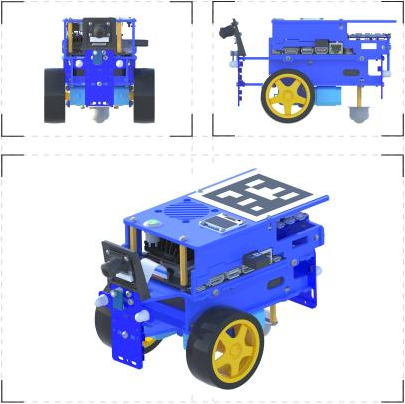
\includegraphics[width=.9\columnwidth]{duckiebot-blue-3d}
    \caption{Duckiebot robot (\url{http://duckietown.org}).}
    \label{fig:duckiebot-3d}
\end{figure}

A consequence of using two independent electric motors in the design of the Duckiebot robot is the way in which the direction of the robot's movement is controlled.
The Duckiebot robot makes turns by changing the speeds of the electric motors depending on which direction it wants to turn and how large the turn radius should be.
Two signals are used to control the robot: $v$-value of the linear speed and $omega$-value of the rotational speed along the robot's vertical Z axis, see Fig. \ref{fig:duckiebot-kinematics}.

\begin{figure}[h]
    \centering
    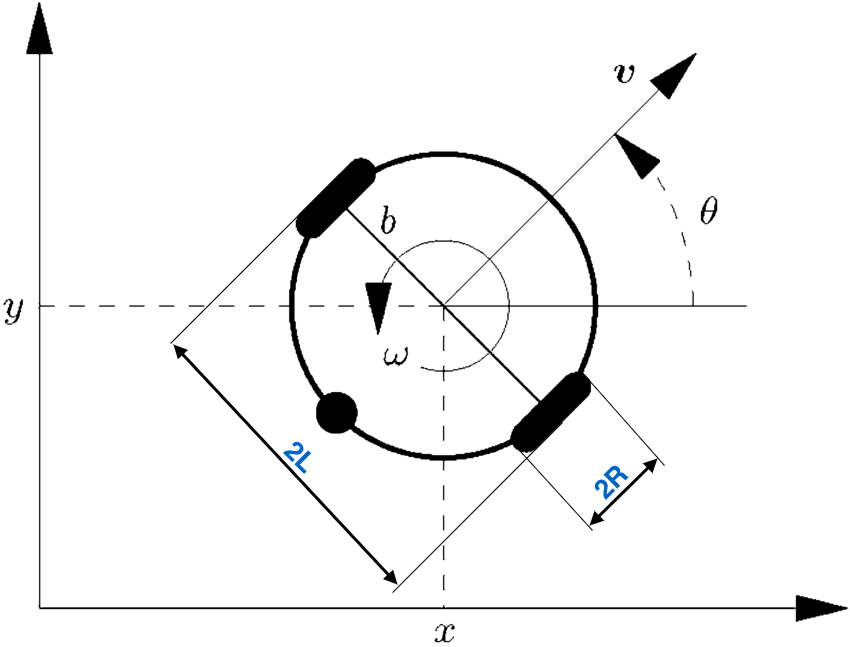
\includegraphics[width=.8\columnwidth]{dt-kinematic}
    \caption{Duckiebot robot kinematic system.}
    \label{fig:duckiebot-kinematics}
\end{figure}

Given the values of $(v, \omega)$ (determined, for example, by the controller), we can calculate the rotational speeds of the robot's wheels from the formulas \eqref{eq:omega-L} and \eqref{eq:omega-R}:

\begin{eqnarray}
	\omega_L & = & \cfrac{v-L\omega}{R} \label{eq:omega-L} \\
	\omega_R & = & \cfrac{v+L\omega}{R} \label{eq:omega-R}
\end{eqnarray}
\\
This type of Duckiebot robot control system is very commonly used in robotics and is called \emph{differential drive} \cite{siegwart2011introduction}. The advantage of such a kinematic system for the motion of the Duckiebot robot is the simplicity of the design (no torsion axis mechanisms of the wheels) while the disadvantage is the need to constantly control the rotational speed of the robot's wheels ($\omega_R$, $\omega_L$) so that it moves along the specified route.

%%%%%%%%%%%%%%%%%%%%%%%%%%%%%%%%%%%%%%%%%%%%%%%%%%%%

\section{Classic implementation with a PID controller}\label{sec:pid-controller}
The classic Duckiebot robot control system uses a PID controller. The task of the control system is to generate such a control signal $u_i$ to minimize the value of the error signal $e_i$, where $i$-consecutive time moments. Figure \ref{fig:pid-pipeline} shows a block diagram of the Duckiebot robot control system using the PID controller and the robot camera as a sensor.

\begin{figure}[h]
    \centering
    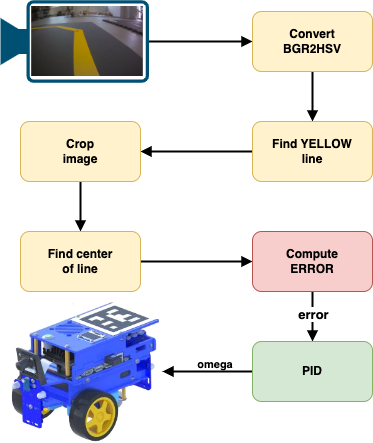
\includegraphics[width=.8\columnwidth]{PipeLinePID}
    \caption{Schematic of Duckiebot robot control system using PID controller.}
    \label{fig:pid-pipeline}
\end{figure}

The error signal $e_i$ is defined as the difference between the center of the vertical axis of the camera image and the point in the analyzed image area containing the line along which the Duckiebot robot should move, see Fig. \ref{fig:error-definition}. 

\begin{figure}[h]
    \centering
    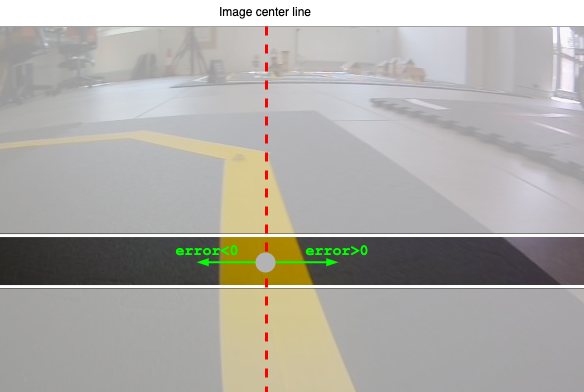
\includegraphics[width=.95\columnwidth]{ErrorDefinition.png}
    \caption{Error determination for the control system implementing the \emph{line follower} functionality for the Duckiebot robot.}
    \label{fig:error-definition}
\end{figure}

The control system of the Duckiebot robot is a discrete system (implemented on JetsoNANO computer), so the discrete version of the PID controller has to be used. Taking into account the drive type of the Duckiebot robot \emph{differential drive robot}, the control signal $u_i$ generated by the PID controller is equivalent to the rotational speed $u_i$ along the Z axis of the robot.

\subsection{PID controller}
One of the best known and most widely used controllers in automatic control systems is the PID controller. This is primarily due to its versatility, ease of implementation in both analog and digital form, and the relatively simple and intuitive way of tuning the PID controller parameters. The discrete version of the PID controller that was used in the Duckietown robot control system is given by the equation \eqref{eq:pid}:

\begin{equation}
u_i = K_p e_i + K_i \sum_{i=0}^k{e_i \Delta t} + K_d \cfrac{e_i-e_{i-1}}{\Delta t}
\label{eq:pid}
\end{equation}
%https://github.com/duckietown/mooc-exercises/blob/c476a67fea9836beab99eed23cfc1a83c77af7bb/modcon/solution/05-PID-Control/PID_controller.ipynb
where: $K_p$ amplification of the proportional part, $K_i$ amplification of the integrating part, $K_d$ amplification of the differentiating part, $e_i$ error at the $i$th instant of time, $\Delta t$ time step \cite{aastrom2021feedback}.

\subsection{Error measurement}
The value of the error signal $e_i$ is determined from the images transmitted by the Duckiebot robot camera. In order to determine the value of the $e_i$ signal, it is necessary to perform several operations on the transmitted images (see Figure \ref{fig:pid-pipeline}). 
The first operation is to convert the image from the RGB color space to the HSV space (\emph{Hue}, \emph{Saturation}, \emph{Value}). This conversion of the color space of images is mainly aimed at better color discrimination and recognition. 
Another operation is to find a line of a certain color in the image along which the Duckiebot robot should move. Such an operation is to leave only the line marking the robot's route in the image and remove all other elements (e.g. background) from the image. 
Next operation is to reduce the area being analyzed by performing a cropping operation. This operation aims to find the exact center of the line along which the Duckiebot robot is to move. 
The center of the line is found as the coordinates of the center of gravity obtained, as a result of the previous transformations, of the line that determines the route of the Duckiebot robot. Figure \ref{fig:img-transformation-summary} shows the result of the specific transformations performed on the robot's camera image to determine the value of the position error $e_i$.

\begin{figure}[hbt!]
    \centering
    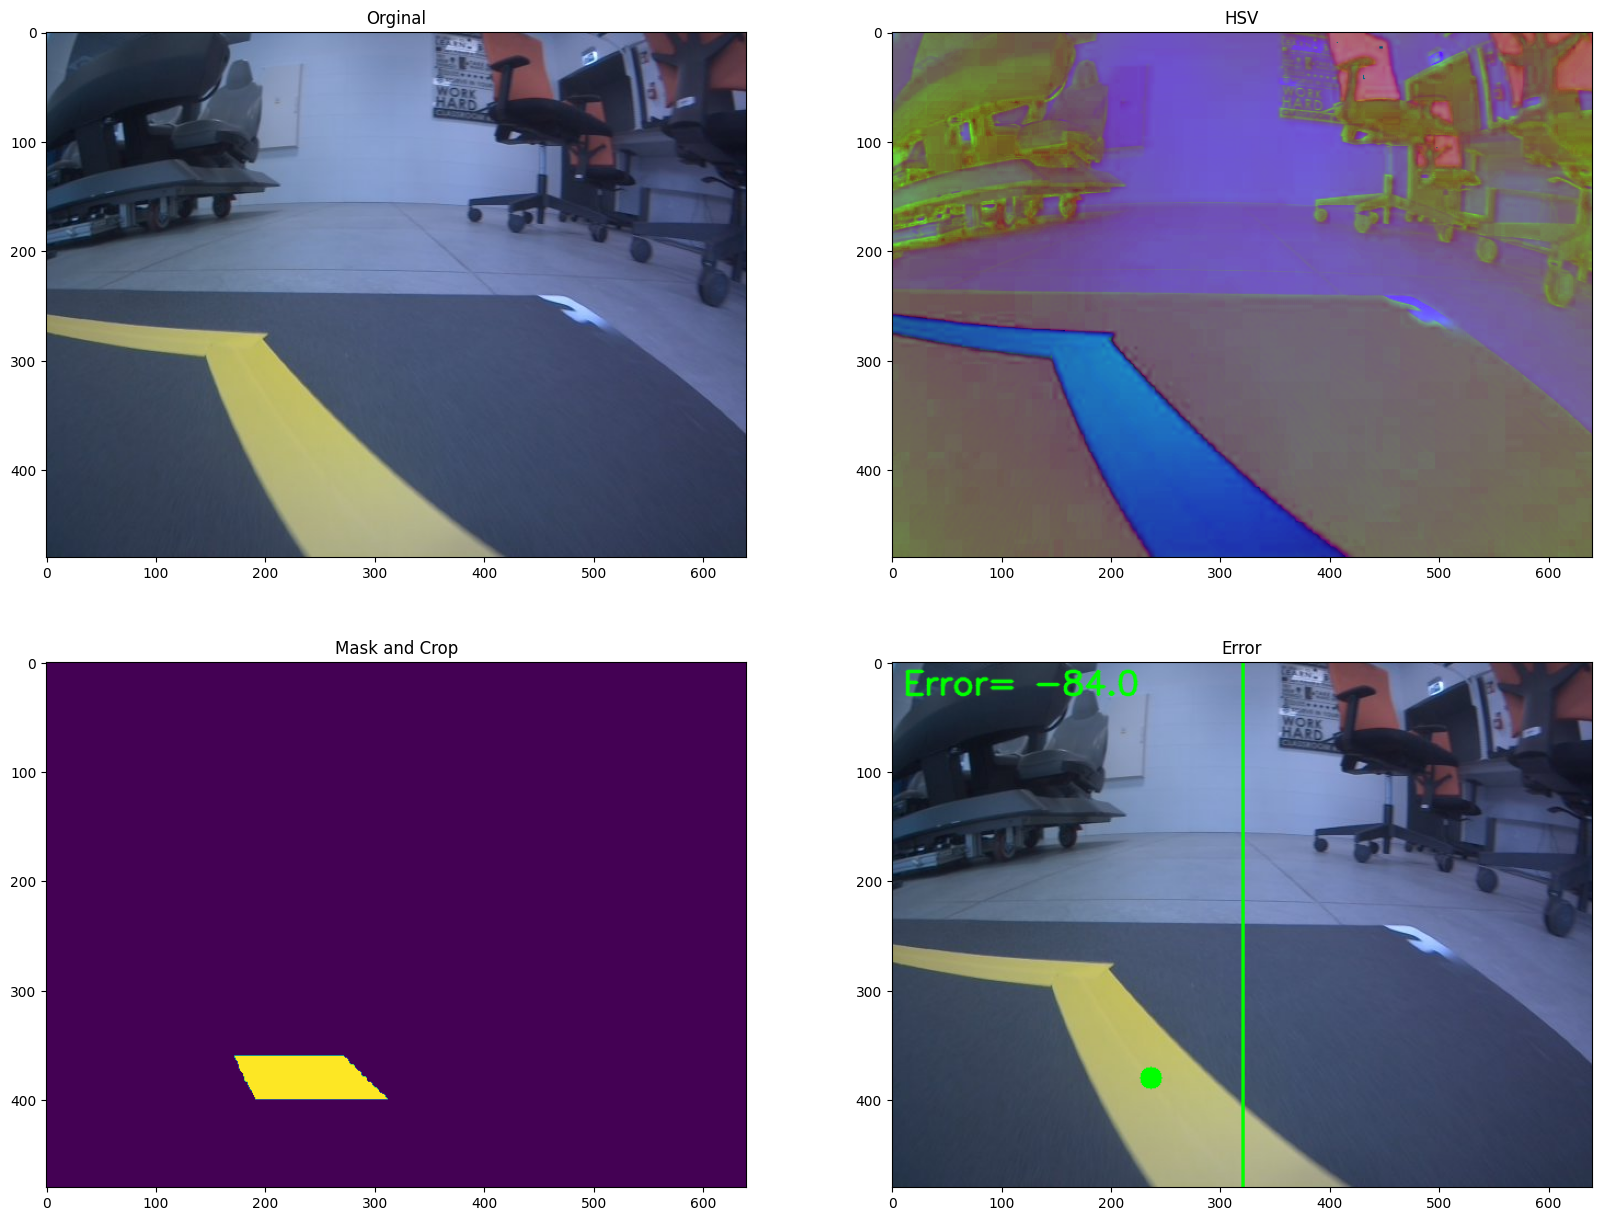
\includegraphics[width=.95\columnwidth]{img-transformation.png}
    \caption{Operations performed on robot camera images to determine position error  $e_i$.}
    \label{fig:img-transformation-summary}
\end{figure}

Finally, the position error value $e_i$ is normalized to the interval $e_i \in [-1;1]$. This is to make independent of the size (width, height) of the images transmitted from the camera.

%%%%%%%%%%%%%%%%%%%%%%%%%%%%%%%%%%%%%%%%%%%%%%%%%%%%

\section{Implementation using neural networks}\label{sec:nn-controller}
The second method of generating a control signal $u_i$ uses a convolutional neural network (\emph{Convolutional Neural Network} CNN). The block diagram of the control system using neural networks is shown in Fig. \ref{fig:cnn-pipeline}.

\begin{figure}[h]
    \centering
    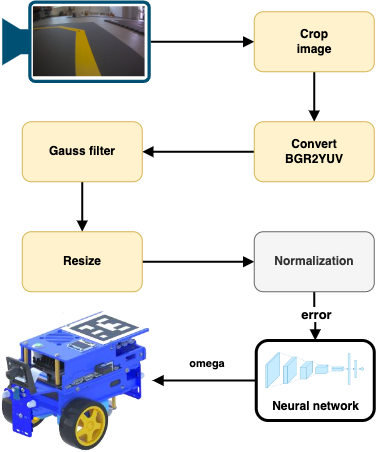
\includegraphics[width=.8\columnwidth]{NNPipeline3}
    \caption{Schematic of Duckiebot robot control system using convolutional neural networks.}
    \label{fig:cnn-pipeline}
\end{figure}

Convolutional neural networks are very effective especially in the tasks of pattern recognition and image processing. CNNs repeatedly use the convolution operation whose use is aimed at extracting characteristic features (edges, textures, shapes) from input images on the basis of which a classical neural network can carry out an inference of "what is in the image." Convolutional neural networks are used in various fields, such as image recognition, text analysis, speech processing, facial recognition, cars, diagnosing diseases from medical images, analyzing satellite images, etc. \cite{li2021survey}, \cite{rawat2017deep}, \cite{almasi2020robust}.

When a CNN is used to control a Duckiebot robot, such a network receives images from the camera as input (after performing several transformations) based on which it generates a $u_i$ control signal which is interpreted as the $\omega_i$ speed along the robot's Z-axis, see Fig. \ref{fig:cnn-pipeline}.

\subsection{Convolutional Neural Network}
The proposed structure of the convolutional neural network is shown in Fig. \ref{fig:cnn-structure} and it should be noted that this is one of the possible network structures that can be used.

\begin{figure}[h]
    \centering
    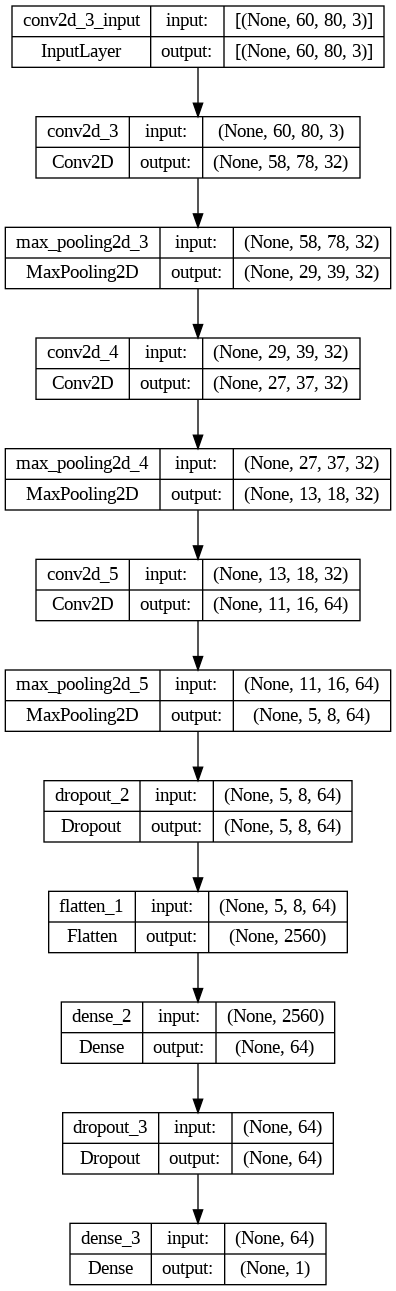
\includegraphics[width=.5\columnwidth]{cnn2}
    \caption{Structure of the convolutional neural network used to control the Duckiebot robot.}
    \label{fig:cnn-structure}
\end{figure}

The network consists of the first convolutional layer, the next layer is the \emph{MaxPooling} layer. Its purpose is to reduce the size of the input data. The next layers of the network are the convolution layer and the \emph{MaxPooling} layer - this arrangement of layers is repeated twice. Each time, the convolution layers extract further features of the input image relevant to the control of the Duckiebot robot, while the \emph{MaxPooling} layers reduce the size of the data. The function of the next layer \emph{Dropout} is randomly turns off individual neurons of the network, so as to prevent the phenomenon of \emph{overfitting} and support the generalization ability of the neural network. Before the data is sent to the input of the actual neural network, it must be flattened, which is the function of the \emph{Flatten} layer. It transforms the multidimensional data into a one-dimensional input vector to the next layer \emph{Dense}. The \emph{Dense} layer is responsible for performing classification, regression or other machine learning tasks. The output of the CNN is the value of the signal $\omega$ in the interval $[-8: ; -8]$ therefore the activation function is from the output of the \emph{Dense} layer is the \emph{tanh} function.

\subsection{Data preparation}
Each neural network is only as good as the good data it was trained with. Hence, a very important step in working with neural networks is to prepare a good set of learning data. In the case of the Duckiebot robot and the task it is supposed to perform (\emph{line follower}), the learning data for the network consists of pairs: the image from the camera and the corresponding correct $\omega$ value, see Fig. \ref{fig:cnn-pipeline}. The data necessary to train the network can be obtained by controlling the Duckiebot robot manually (e.g., with a gamepad) or by using a previously developed control system with a PID controller by adding a script that writes the data into log file. 

In addition to the appropriate amount of logged data for learning the neural network, it is important that the data is sufficiently diverse - that is, that it covers the largest possible number of cases, situations, events in which the Duckiebot robot may find itself. Figure \ref{fig:cnn-data-hist1} shows a histogram of an example dataset that has been logged. 

\begin{figure}[h]
	\begin{subfigure}{.475\columnwidth}
    	\centering
    	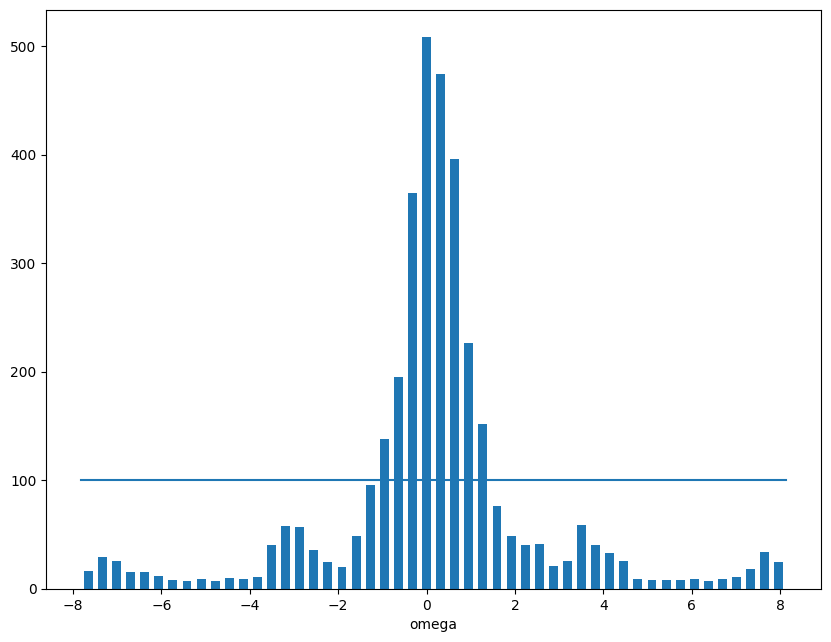
\includegraphics[width=1\columnwidth]{h1}
    	\caption{}
    	\label{fig:cnn-data-hist1}
    \end{subfigure}
    \begin{subfigure}{.475\columnwidth}
    	\centering
    	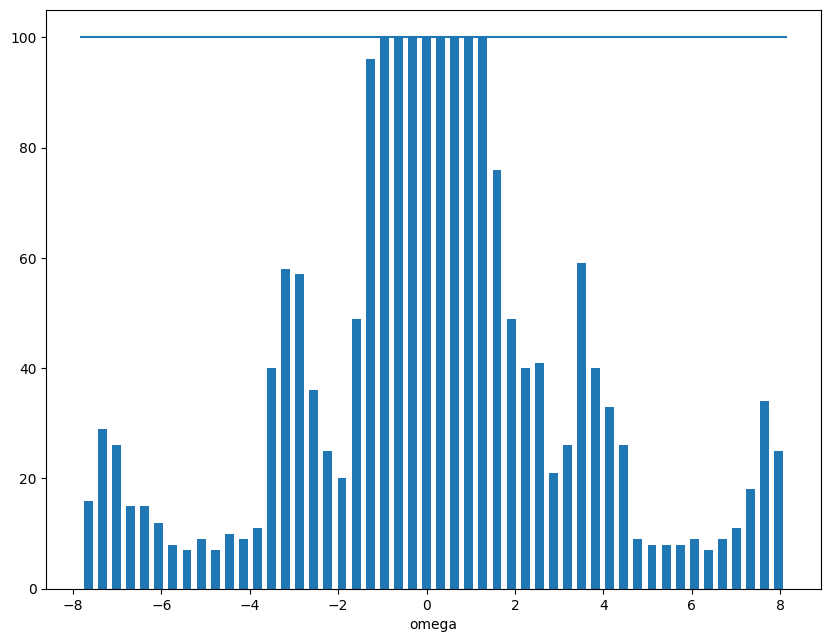
\includegraphics[width=1\columnwidth]{h2}
    	\caption{}
    	\label{fig:cnn-data-hist2}
    \end{subfigure}
    
    \caption{Histogram of logged data before analysis (a) and after analysis (b).}
    \label{fig:cnn-data-hist}
\end{figure}

It can be clearly seen that the dominant value in this dataset for the $\omega$ variable is close to $0$, and if you use such data to train a CNN that is supposed to control the Duckiebot robot, it is likely that the robot would drive straight very well, while it would have problems with turns. In such a case, after analyzing the data, one should remove from the learning set data whose values significantly dominate over other values obtaining a more representative learning data set, see Fig. \ref{fig:cnn-data-hist2}.

Similar to the control of the Duckiebot robot using the PID controller, it is necessary to adequately prepare the camera images when controlling the Duckiebot robot using neural networks. The various stages of processing Duckiebot robot camera images are shown in Figure \ref{fig:cnn-pipeline} (yellow-colored blocks) and are: cropping the image to the area of interest, conversion to YUV color space (Y-luminance, UV-color, chrominance), filtering using the Gauus filter, resizing the image and normalizing the values of individual image channels to the interval $[0;1]$. The result of the various operations can be seen in Figure \ref{fig:cnn-image-prepare}.

\begin{figure}[h]
    \centering
    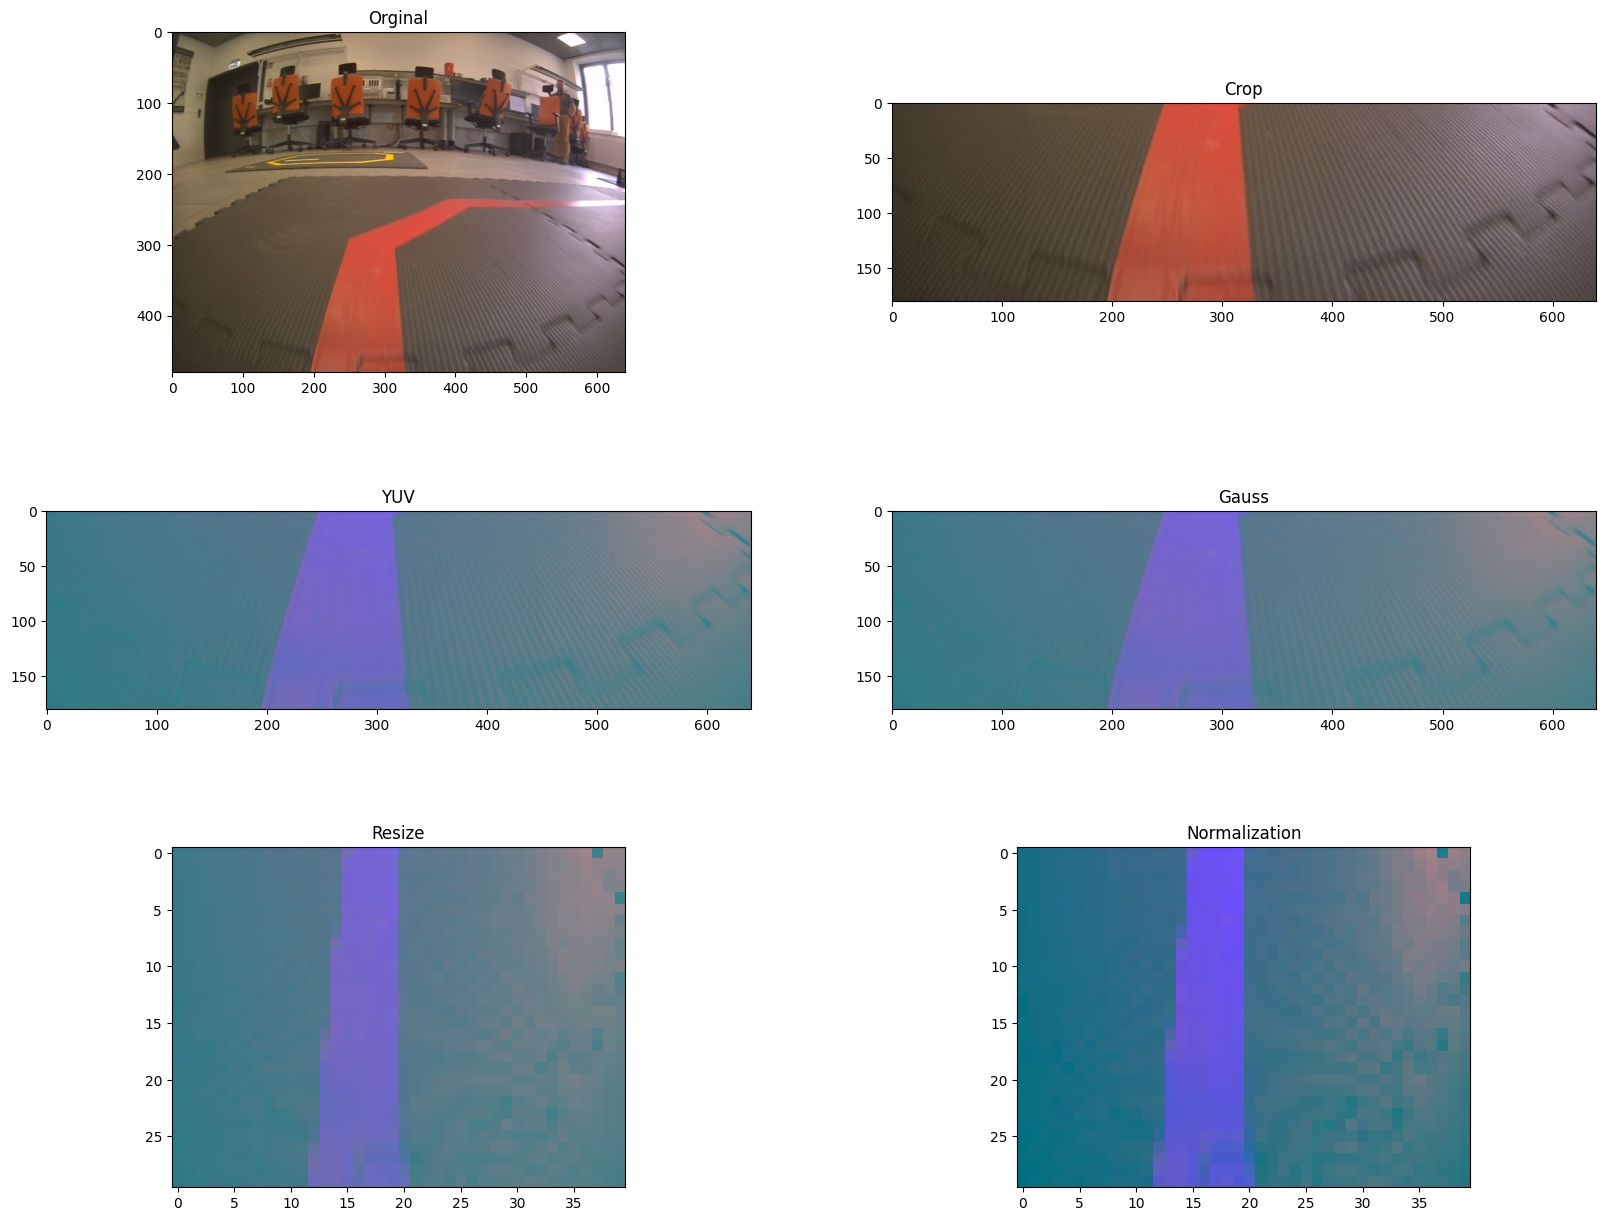
\includegraphics[width=.95\columnwidth]{nn_prepare_image}
    \caption{Operations performed on images from the camera of the Duckiebot robot controlled before the application of the CNN controller.}
    \label{fig:cnn-image-prepare}
\end{figure}

%%%%%%%%%%%%%%%%%%%%%%%%%%%%%%%%%%%%%%%%%%%%%%%%%%%%

\section{Practical advice}\label{sec:practical-info}
The Duckietown robot software was implemented using the Robot Opertion System framework (\emph{ROS}) \cite{quigley2015programming}. It is currently one of the most popular frameworks for programming robots of various kinds. The consequence of choosing the ROS framework is the choice of programming language, and in the case of Duckiebot robots it is Python. The Duckietown project also defines how to develop custom software for robots and enforces the use of containerization technology. This is a very good practice in accordance with the software development trends of the time. A detailed description together with examples of creating software for Duckie robots is very well described in the documentation of the project \cite{Daniele:ff}. 
The use of the ROS framework also makes it possible to efficiently create and test software without having to constantly upload new versions to the Duckiebot robot. By configuring the host computer appropriately so that it connects to the ROS server running on the selected Duckiebot robot, you can implement and test your own software conveniently and efficiently, see Fig. \ref{fig:env-develop}.

\begin{figure}[h]
    \centering
    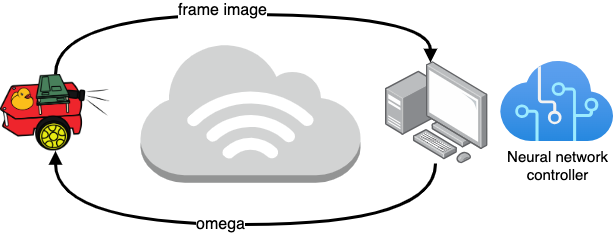
\includegraphics[width=.8\columnwidth]{controll_schema2}
    \caption{Setting up a development environment for the Duckiebot robot.}
    \label{fig:env-develop}
\end{figure}

The proposed controllers should be implemented as ROS nodes. The nodes should read images from the robot's camera (sent as ROS messages) and generate a $\omega$ control signal as output. To simplify the control of the Duckiebot robot, it can be assumed that it moves at a constant linear speed $v=const$.

Convolutional neural networks can be created, trained and tested using the \emph{keras} and \emph{tensorflow} modules of the Python language. The advantage of the \emph{keras} and \emph{tensorflow} modules is also very good documentation with a very large number of examples. 

It is also necessary to pay attention to the correct preparation of data for learning neural networks, each camera image must correspond to a single, correct value of the $\omega$ signal.

%%%%%%%%%%%%%%%%%%%%%%%%%%%%%%%%%%%%%%%%%%%%%%%%%%%%

\section{Conclusions}\label{sec:conclusion}
The PID controller is used successfully in many control systems and its implementation is relatively simple. There are also a number of methods and algorithms for adjusting controller parameters for this type of controller. PID controllers are also not free of disadvantages. One of them is the requirement to know, even roughly, the model of the process we want to control. Thus, there is a need to identify both the structure of the process model and its parameters. Identification tasks are not simple tasks, requiring a great deal of knowledge about the nature of the process itself. There are also methods for identifying process models based on the results of practical experiments, but in this case it may not always be possible to conduct such an experiment. When using a PID controller, one should also be aware that it was developed for processes whose operation can be described by linear models. Unfortunately, the behavior of the vast majority of dynamic systems is described by nonlinear models. The consequence of this is that in such a case the PID controller works using linear approximations of nonlinear systems - which can cause various errors, inaccuracies, etc.

Unlike the classic PID controller, controllers using artificial neural networks do not need to know the mathematical model of the process they control and its parameters. The ability to design different neural network architectures, such as convolutional, recurrent or deep neural networks, makes it possible to adapt the neural regulator to the specific process it is supposed to control. On the other hand, the multiplicity of neural network architectures, their design means that we can never be sure whether a given neural network structure is optimal.
The selection of parameters of neural controllers is done automatically by using appropriate network learning algorithms.  The key element influencing the correctness of neural regulator operation is the data that the learned neural network is. The disadvantage of regulators using neural networks is the inability to demonstrate the stability of operation of the systems they control. In the case of the PID regulator, despite the use of approximate models of the process, it is very often possible to prove that a closed control system will operate stably in any or a certain range of values of variables. Unfortunately, such an analysis cannot be carried out in the case of neural regulators. 

In summary, the implementation of two different controllers to perform the same task provides an opportunity to learn the advantages and disadvantages of each. Students, in the course of solving the problem posed, must demonstrate theoretical knowledge of the issues and, which is particularly important for engineers, acquire the ability to practically apply theoretical knowledge. 


\bibliographystyle{IEEEtran}
\bibliography{references}

\end{document}
